\documentclass[11pt, a4paper]{article} % setsfont size and layout

%% required packages %%

\usepackage[margin=2.5cm]{geometry} % margins
\usepackage[utf8]{inputenc} % Umlaute
\usepackage{amsmath,amssymb, physics}		% math formulas
\usepackage{graphicx}		% graphics
\usepackage{fancyhdr}		% header and footer on every page
\usepackage{setspace}		% line space (e.g. \singlespacing, \onehalfspacing or \doublespacing)
\usepackage{cancel}
\usepackage{braket}
\usepackage{xcolor}
%% Here the main part of the document begins %%

\begin{document}
	
%% Some more settings %%
	
\setlength{\parindent}{0pt} % first line in paragraph will not be indented
\onehalfspacing				% 1.5 line spacing
%\thispagestyle{empty}		% no header and page number on first page


%% Header on first page with course information etc. %%
%\begin{tabular}{p{15.5cm}}
%	{\large \textbf{Classical Mechanics}} \\
%	Westlake University \\ 
%	\hline
%	\\
%\end{tabular}

\vspace*{0.1cm}				% vertical space between header on top of the page and main heading


\begin{center}
	{\Large \textbf{Classical Mechanics}}
    \vspace*{2mm}
    
    {\Large \textbf{Final Exam}}
	\vspace{8mm}
%Name: 
%\end{center} 
%\vspace{0.1cm}

{\Large \bf \color{red} Time: 2:00 - 4:00 pm, Dec. 30th, 2025}
\vspace*{2mm}

{\Large \bf \color{red} Duration: 120 minutes}
\vspace*{2mm}

{\Large \bf \color{red} Total Points: 100 out of 110}
\end{center}
\vspace*{8mm}

{\Large \bf \color{orange} Instruction:} 
\vspace*{2mm}

{\Large \bf \color{orange} \hspace{2em} This is a closed-book exam; no aids are allowed.}
\vspace*{2mm}

{\Large \bf \color{orange} \hspace{2em} Total 11 pages including the front page of the instruction.}
\vspace*{2mm}

{\Large \bf \color{orange} \hspace{2em} Provide relevant mathematical steps.} 
\vspace*{2mm}

{\Large \bf \color{orange} \hspace{2em} All answers must be in English.}
\vspace*{2mm}

{\Large \bf \color{orange} \hspace{2em} Don't open the booklet before the exam begins.}
\vspace{5cm}

\begin{center}
{\Large \bf Student Name: \underline{\hbox to 40mm{}}}
\vspace*{8mm}

{\Large \bf Student ID: \underline{\hbox to 40mm{}}}
\vspace*{2mm}
\end{center}

\newpage
\section*{Problem 1 [$5 + 5$ points]} 
\begin{enumerate}
  \item[(1)] Write down Newton’s second law, the Euler-Lagrange equation, and Hamilton’s equations of motion. 

  \item[(2)] State the principle of virtual work for a mechanical system in static equilibrium. Starting from Newton’s second law, derive the principle of virtual work.

  \end{enumerate}

\subsection*{Answer}
\subsubsection*{(1) Fundamental Equations [5 points]}

\begin{description}
    \item[A. Newton's Second Law] \hfill \textbf{[1 point]}
    \begin{itemize}
        \item Equation: $\mathbf{F} = \frac{d\mathbf{p}}{dt}$ or $\mathbf{F} = m\mathbf{a}$ (or $\mathbf{F} = m\ddot{\mathbf{r}}$).
        \item \textit{Note:} Vector notation ($\mathbf{F}, \mathbf{a}$) or component index notation ($F_i = m \ddot{x}_i$) is required. If scalar form is written without context, deduct 0.5 points.
    \end{itemize}

    \item[B. Euler-Lagrange Equation] \hfill \textbf{[2 points]}
    \begin{itemize}
        \item Equation: $\frac{d}{dt}\left(\frac{\partial L}{\partial \dot{q}_i}\right) - \frac{\partial L}{\partial q_i} = 0$ (for $i = 1, \dots, n$).
    \end{itemize}

    \item[C. Hamilton's Equations of Motion] \hfill \textbf{[2 points]}
    \begin{itemize}
        \item Equations: 
        \begin{align*}
            \dot{q}_i &= \frac{\partial H}{\partial p_i} \\
            \dot{p}_i &= -\frac{\partial H}{\partial q_i}
        \end{align*}
    \end{itemize}
\end{description}

\subsubsection*{(2) Principle of Virtual Work [5 points]}

\begin{description}
    \item[A. Statement of the Principle] \hfill \textbf{[2 point]}
    
    For a system in static equilibrium, the virtual work of the \textbf{applied forces} vanishes for any arbitrary virtual displacement consistent with the constraints.

    \item[B. Derivation] \hfill \textbf{[3 points]}
    \begin{enumerate}
        \item \textbf{Expansion of Virtual Displacement and work} \hfill \textbf{[1 point]} \\
        Express $\delta \vec{r}$ in terms of generalized coordinates $q_i$:
        $$ \delta \vec{r} = \sum_i \frac{\partial \vec{r}}{\partial q_i} \delta q_i + \xcancel{\frac{\partial \vec{r}}{\partial t} \delta t} $$
        Substitute $\delta \vec{r}$ into the work equation $\delta W = \vec{F}_{net} \cdot \delta \vec{r}$ to define the net generalized force $Q_i^{net}$:
        $$ \delta W = \sum_i \left( \vec{F}_{net} \cdot \frac{\partial \vec{r}}{\partial q_i} \right) \delta q_i = \sum_i Q_i^{net} \delta q_i $$
        \textit{Criteria:} Must explicitly show or mention that the time term is zero (frozen time) or write the sum directly without $dt$.
        
        \item \textbf{Decomposition of Forces} \hfill \textbf{[1 point]} \\
        Split the net generalized force into Constraint ($Q^c$) and Applied ($Q$) parts:
        $$ Q_i^{net} = Q_i^c + Q_i $$
        $$ \sum_i (Q_i^c + Q_i) \delta q_i = 0 \quad (\text{since equilibrium } \delta W_{net}=0) $$

        \item \textbf{Constraint Assumption \& Result} \hfill \textbf{[1 point]} \\
        Argue that for ideal constraints, the work done by constraint forces is zero ($\sum Q_i^c \delta q_i = 0$), leading to the final result:
        $$ \implies \boxed{\sum_i Q_i \delta q_i = 0} $$
    \end{enumerate}
\end{description}



\newpage 
\section*{Problem 2 [$4+3+3$ points]} 
Let the Lagrangian of a system be given by $L(q_k, \dot{q}_k, t)$, where $q_k$ and $\dot{q}_k$ denote the generalized coordinates and velocities, respectively, for $k = 1, \dots, n$. 
The Hamiltonian function is then defined as
\[
H(q_k, p_k, t) = \sum_{k=1}^n p_k \dot{q}_k - L(q_k, \dot{q}_k, t),
\]
where the velocities $\dot{q}_k$ are to be considered as functions of $(q_k, p_k, t)$, implicitly defined via the Legendre transformation.

\begin{enumerate}
  \item[(1)] Compute the total differential $\dd H$ of the Hamiltonian. Express your result in terms of the differentials $\dd q_k$, $\dd p_k$, $\dd\dot{q}_k$, and $\dd t$. 
  
  \item[(2)] Using the result of (1), derive Hamilton's equations of motion.
  
  \item[(3)] Prove that if the Lagrangian $L(q_k, \dot{q}_k)$ does not depend explicitly on time $t$, then the Hamiltonian $H$ is conserved.

\end{enumerate}
\subsection*{Answer}

\subsubsection*{(1) Total Differential of $H$ (4 points)}
\begin{itemize}
    \item Expand the differential of the product term $\sum p_k \dot{q}_k$ and the total differential of the Lagrangian $L(q, \dot{q}, t)$:
    \[
    dH = \sum_k (p_k d\dot{q}_k + \dot{q}_k dp_k) - \sum_k \left( \frac{\partial L}{\partial q_k} dq_k + \frac{\partial L}{\partial \dot{q}_k} d\dot{q}_k \right) - \frac{\partial L}{\partial t} dt
    \]
    \hfill \textbf{(2 points)} \\
    \textit{(1 point for correctly expanding $d(p\dot{q})$, 1 point for expanding $dL$)}

    \item Use the definition of generalized momentum $p_k = \frac{\partial L}{\partial \dot{q}_k}$ to show that the terms involving $d\dot{q}_k$ cancel out:
    \[
    \sum_k p_k d\dot{q}_k - \sum_k \frac{\partial L}{\partial \dot{q}_k} d\dot{q}_k = 0
    \]
    \hfill \textbf{(1 point)}

    \item Substitute Lagrange's equations $\dot{p}_k = \frac{\partial L}{\partial q_k}$ to arrive at the final expression:
    \[
    dH = \sum_{k=1}^n \left( \dot{q}_k dp_k - \dot{p}_k dq_k \right) - \frac{\partial L}{\partial t} dt
    \]
    \hfill \textbf{(1 point)}
\end{itemize}

\subsubsection*{(2) Hamilton's Equations (3 points)}
\begin{itemize}
    \item State the mathematical total differential of $H$ considered as a function of $(q_k, p_k, t)$:
    \[
    dH = \sum_{k=1}^n \left( \frac{\partial H}{\partial q_k} dq_k + \frac{\partial H}{\partial p_k} dp_k \right) + \frac{\partial H}{\partial t} dt
    \]
    \hfill \textbf{(1 point)}

    \item Compare the coefficients of the differentials $dq_k$, $dp_k$, and $dt$ with the result from Part (1):
    \hfill \textbf{(1 point)}

    \item Write down the final canonical equations (Hamilton's equations):
    \[
    \dot{q}_k = \frac{\partial H}{\partial p_k}, \quad \dot{p}_k = -\frac{\partial H}{\partial q_k}, \quad \left( \text{and } \frac{\partial H}{\partial t} = -\frac{\partial L}{\partial t} \right)
    \]
    \hfill \textbf{(1 point)}
\end{itemize}

\subsubsection*{(3) Conservation of Hamiltonian (3 points)}
\begin{itemize}
    \item Write the total time derivative of $H(q_k, p_k, t)$:
    \[
    \frac{dH}{dt} = \sum_{k=1}^n \left( \frac{\partial H}{\partial q_k} \dot{q}_k + \frac{\partial H}{\partial p_k} \dot{p}_k \right) + \frac{\partial H}{\partial t}
    \]
    \hfill \textbf{(1 point)}

    \item Substitute Hamilton's equations ($\dot{q}_k = \partial H/\partial p_k$ and $\dot{p}_k = -\partial H/\partial q_k$) into the summation, showing that the terms cancel each other out:
    \[
    \sum_{k=1}^n \left( \frac{\partial H}{\partial q_k} \frac{\partial H}{\partial p_k} - \frac{\partial H}{\partial p_k} \frac{\partial H}{\partial q_k} \right) = 0
    \]
    \hfill \textbf{(1 point)}

    \item Conclude that since $L$ does not depend explicitly on time, $\frac{\partial L}{\partial t} = 0 \implies \frac{\partial H}{\partial t} = 0$, therefore:
    \[
    \frac{dH}{dt} = 0 \quad (\text{H is conserved})
    \]
    \hfill \textbf{(1 point)}
\end{itemize}

\newpage
\section*{Problem 3 [$10$ points]}
A bead of mass $m$ slides on a frictionless rod inclined at a constant angle $\alpha$ to the vertical axis. The rod rotates about this vertical axis with a constant angular velocity $\omega$. Gravity $g$ acts vertically downwards. Derive the equation of motion for the position $r$ of the bead along the rod using the Lagrangian formalism. 
\begin{figure}[h]
    \centering
    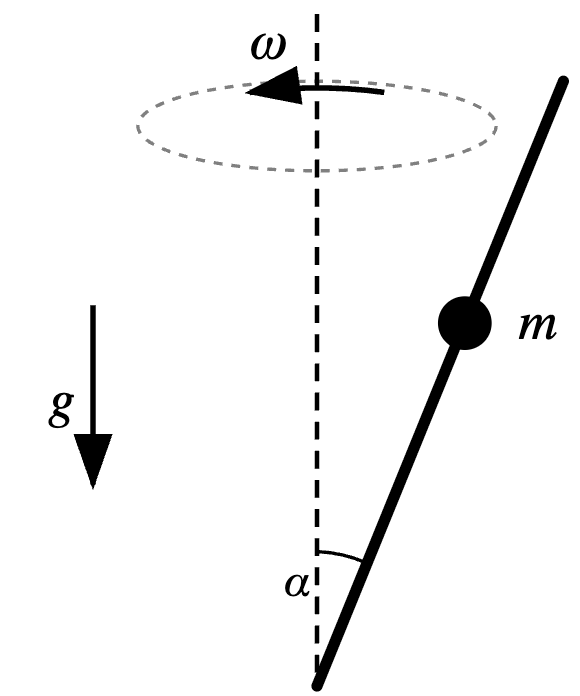
\includegraphics[width=0.35\textwidth]{bead.png}
    \label{P7}
\end{figure}

\subsection*{Answer}

\subsubsection*{(a) Lagrangian Formulation (5 points)}
\begin{itemize}
    \item \textbf{Kinetic Energy ($T$):} Identify the velocity components. The radial velocity is $\dot{r}$ and the tangential velocity due to rotation is $\omega(r \sin \alpha)$.
    \[
    T = \frac{1}{2}m v^2 = \frac{1}{2}m \left( \dot{r}^2 + (\omega r \sin \alpha)^2 \right)
    \]
    \hfill \textbf{(2 points)} \\

    \item \textbf{Potential Energy ($V$):} Define the gravitational potential energy based on the height $h = r \cos \alpha$ (assuming $V=0$ at $r=0$).
    \[
    V = m g r \cos \alpha
    \]
    \hfill \textbf{(2 points)}

    \item \textbf{The Lagrangian ($L$):} Construct the Lagrangian $L = T - V$.
    \[
    L = \frac{1}{2}m(\dot{r}^2 + \omega^2 r^2 \sin^2 \alpha) - m g r \cos \alpha
    \]
    \hfill \textbf{(1 point)}
\end{itemize}

\subsubsection*{(b) Equation of Motion (5 points)}
\begin{itemize}
    \item \textbf{Derivatives:} Calculate the necessary partial derivatives for the Euler-Lagrange equation $\frac{d}{dt}(\frac{\partial L}{\partial \dot{r}}) - \frac{\partial L}{\partial r} = 0$.
    \[
    \frac{\partial L}{\partial \dot{r}} = m\dot{r} \implies \frac{d}{dt}\left(\frac{\partial L}{\partial \dot{r}}\right) = m\ddot{r}
    \]
    \[
    \frac{\partial L}{\partial r} = m \omega^2 r \sin^2 \alpha - m g \cos \alpha
    \]
    \hfill \textbf{(3 points)} \\

    \item \textbf{Final Equation:} Assemble and rearrange the terms to obtain the final equation of motion.
    \[
    m\ddot{r} - (m \omega^2 r \sin^2 \alpha - m g \cos \alpha) = 0
    \]
    \[
    \implies m\ddot{r} = m \omega^2 r \sin^2 \alpha - m g \cos \alpha
    \]
    \hfill \textbf{(2 points)} \\
\end{itemize}

\newpage
\section*{Problem 4 [$10$ points]}
A block of mass $m$ is held motionless on a frictionless plane of mass $M$ and angle of inclination $\theta$ (see the Figure below). The plane rests on a frictionless horizontal surface. The block is released. What is the horizontal acceleration of the plane of mass $M$?

\begin{figure}[h]
    \centering
    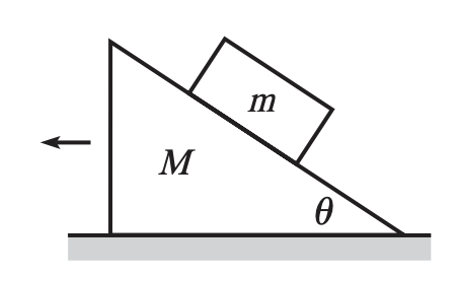
\includegraphics[width=0.4\textwidth]{Finala_P7.png}
    \label{P7}
\end{figure}

\subsection*{Answer}

\subsubsection*{(1) Setup and Lagrangian Construction (4 points)}
\begin{itemize}
    \item \textbf{Coordinate Definition \& Constraints:} 
    Define coordinates $x_1$ (horizontal position of wedge $M$, positive left) and $x_2$ (horizontal position of block $m$, positive right). Establish the kinematic constraint for the vertical motion of the block: 
    \[ y = (x_1 + x_2) \tan \theta \implies v_y = (\dot{x}_1 + \dot{x}_2) \tan \theta \]
    \hfill \textbf{(1 point)}
    
    \item \textbf{Kinetic Energy ($T$):} 
    Write the kinetic energy for the plane $M$ and the block $m$. Note that the block's velocity has both horizontal component $\dot{x}_2$ and vertical component $v_y$.
    \[ T = \frac{1}{2} M \dot{x}_1^2 + \frac{1}{2} m \left( \dot{x}_2^2 + (\dot{x}_1 + \dot{x}_2)^2 \tan^2 \theta \right) \]
    \hfill \textbf{(1 point)}
    
    \item \textbf{Potential Energy ($V$):} 
    Define the potential energy. Assuming $y$ is measured downwards from the top, potential decreases as the block slides down: $V = -mg y = -mg(x_1 + x_2)\tan\theta$. (Or equivalently, write the Work term $W = mg y$ if using $L=T+W$ convention as implied by the reference sign).
    \hfill \textbf{(1 point)}
    
    \item \textbf{The Lagrangian ($L$):} 
    Combine to form the final Lagrangian $L = T - V$:
    \[ L = \frac{1}{2} M \dot{x}_1^2 + \frac{1}{2} m \left[ \dot{x}_2^2 + (\dot{x}_1 + \dot{x}_2)^2 \tan^2 \theta \right] + mg(x_1 + x_2) \tan \theta \]
    \hfill \textbf{(1 point)}
\end{itemize}

\subsubsection*{(2) Equations of Motion (2 points)}
\begin{itemize}
    \item Apply the Euler-Lagrange equation $\frac{d}{dt}\frac{\partial L}{\partial \dot{q}} - \frac{\partial L}{\partial q} = 0$ for $x_1$ and $x_2$ to obtain the coupled differential equations:
    \begin{align*}
        x_1: & \quad M\ddot{x}_1 + m(\ddot{x}_1 + \ddot{x}_2)\tan^2\theta = mg\tan\theta \\
        x_2: & \quad m\ddot{x}_2 + m(\ddot{x}_1 + \ddot{x}_2)\tan^2\theta = mg\tan\theta
    \end{align*}
    \hfill \textbf{(2 points)} \\
\end{itemize}

\subsubsection*{(3) Solving for Acceleration (4 points)}
\begin{itemize}
    \item \textbf{Decoupling / Conservation of Momentum:} 
    Subtract the two equations of motion (or recognize horizontal momentum conservation) to find the relationship between accelerations:
    \[ M\ddot{x}_1 - m\ddot{x}_2 = 0 \implies \ddot{x}_2 = \frac{M}{m}\ddot{x}_1 \]
    \hfill \textbf{(2 points)}
    
    \item \textbf{Final Calculation:} 
    Substitute $\ddot{x}_2$ back into the first equation of motion and solve for $\ddot{x}_1$:
    \[ M\ddot{x}_1 + m\left( \ddot{x}_1 + \frac{M}{m}\ddot{x}_1 \right)\tan^2\theta = mg\tan\theta \]
    Factor out $\ddot{x}_1$ and use trigonometric identities ($\tan^2\theta + 1 = \sec^2\theta$) to simplify:
    \[ \ddot{x}_1 \left[ M + (M+m)\tan^2\theta \right] = mg\tan\theta \]
    \[ \implies \ddot{x}_1 = \frac{mg \sin \theta \cos \theta}{M + m \sin^2 \theta} \]
    \hfill \textbf{(2 points)}
\end{itemize}

\newpage
\section*{Problem 5 [$5+5$ points]}
A system with one degree of freedom has Hamiltonian 
\begin{equation*}
    H(q,p) = \frac{p^2}{2m} + A(q)p + B(q)
\end{equation*}
where $A$ and $B$ are certain functions of the coordinate $q$, and $p$ is the momentum.

\begin{enumerate}
\item[(1)] Find the generalized velocity $\dot{q}$.

\item[(2)]  Find the Lagrangian $L(q, \dot{q})$.
\end{enumerate}

\subsection*{Answer}

\subsubsection*{(1) Generalized Velocity $\dot{q}$ (5 points)}
\begin{itemize}
    \item \textbf{Hamilton's Canonical Equation:} State or use the correct canonical equation relating generalized velocity to the Hamiltonian.
    \[
    \dot{q} = \frac{\partial H}{\partial p}
    \]
    \hfill \textbf{(2 points)}
    \item \textbf{Differentiation:} Perform the partial differentiation of the given Hamiltonian $H(q,p) = \frac{p^2}{2m} + A(q)p + B(q)$ with respect to momentum $p$.
    \[
    \frac{\partial}{\partial p}\left( \frac{p^2}{2m} + A(q)p + B(q) \right) = \frac{2p}{2m} + A(q)
    \]
    \hfill \textbf{(2 points)}
    \item \textbf{Final Result:} Write down the final expression for the generalized velocity.
    \[
    \dot{q} = \frac{p}{m} + A(q)
    \]
    \hfill \textbf{(1 point)}
\end{itemize}

\subsubsection*{(2) The Lagrangian $L(q, \dot{q})$ (5 points)}
\begin{itemize}
    \item \textbf{Legendre Transformation Definition:} State the definition of the Lagrangian in terms of the Hamiltonian and generalized velocity.
    \[
    L(q, \dot{q}) = p\dot{q} - H(q, p)
    \]
    \hfill \textbf{(1 point)}
    \item \textbf{Inversion of Momentum:} Solve the result from Part (1) to express the momentum $p$ as a function of generalized velocity $\dot{q}$ (since $L$ must be a function of $q$ and $\dot{q}$, not $p$).
    \[
    \dot{q} = \frac{p}{m} + A(q) \implies p = m(\dot{q} - A(q))
    \]
    \hfill \textbf{(1 point)}
    \item \textbf{Substitution:} Substitute the expression for $p$ and the original $H$ into the Legendre transformation formula.
    \begin{align*}
        L &= p\dot{q} - \left( \frac{p^2}{2m} + A(q)p + B(q) \right) \\
          &= p(\dot{q} - A(q)) - \frac{p^2}{2m} - B(q)
    \end{align*}
    Substitute $p = m(\dot{q} - A)$:
    \[
    L = m(\dot{q} - A)(\dot{q} - A) - \frac{[m(\dot{q} - A)]^2}{2m} - B(q)
    \]
    \hfill \textbf{(2 points)} \\
    \item \textbf{Simplification and Final Result:} Simplify the expression to obtain the final Lagrangian.
    \[
    L = m(\dot{q} - A)^2 - \frac{1}{2}m(\dot{q} - A)^2 - B(q)
    \]
    \[
    L(q, \dot{q}) = \frac{1}{2}m(\dot{q} - A(q))^2 - B(q)
    \]
    \hfill \textbf{(1 point)}
\end{itemize}

\newpage
\section*{Problem 6 [$10$ points]}
Consider a one-dimensional harmonic oscillator with Hamiltonian:
\begin{equation*}
    H(q, p) = \frac{1}{2}\left(p^2 + \omega^2 q^2\right),
\end{equation*}
where $q$ and $p$ are the generalized coordinate and momentum, respectively, and $\omega$ is the angular frequency. Let the generating function of the canonical transformation be of type I (a function of the old coordinate $q$ and the new coordinate $Q$), given by:
\begin{equation*}
    F_1(q, Q) = \frac{1}{2} \omega q^2 \cot(2\pi Q).
\end{equation*}

\begin{enumerate}
    \item[(1)] Determine the new Hamiltonian $K(Q, P)$ by performing the canonical transformation defined by the generating function $F_1(q, Q)$. Hint: $p=\frac{\partial F_1}{\partial q}$ and $P=-\frac{\partial F_1}{\partial Q}$.

    \item[(2)] Express the time evolution of the original variables $q(t)$ and $p(t)$ in terms of the new canonical momentum $P$, the frequency $\omega$, and time $t$.
\end{enumerate}

\subsection*{Answer}
\subsubsection*{(1) New Hamiltonian $K(Q, P)$ (5 points)}
\begin{itemize}
    
    \item \textbf{Calculate Derivatives:}
    Compute the partial derivatives explicitly. Note the chain rule for the $\cot(2\pi Q)$ term. (Using Hint)
    \[ p = \frac{\partial}{\partial q}\left(\frac{1}{2} \omega q^2 \cot(2\pi Q)\right) = \omega q \cot(2\pi Q) \]
    \[ P = -\frac{\partial}{\partial Q}\left(\frac{1}{2} \omega q^2 \cot(2\pi Q)\right) = -\frac{1}{2}\omega q^2 \left[ -2\pi \csc^2(2\pi Q) \right] = \pi \omega q^2 \csc^2(2\pi Q) \]
    \hfill \textbf{(2 points)} \\

    \item \textbf{Inversion and Substitution:}
    Invert the relations to express $q$ and $p$ in terms of $Q$ and $P$, or substitute terms directly into the Hamiltonian.
    From the expression for $P$: $\omega^2 q^2 = \frac{\omega P}{\pi} \sin^2(2\pi Q)$.
    Then for momentum: $p^2 = (\omega q \cot(2\pi Q))^2 = \frac{\omega P}{\pi} \cos^2(2\pi Q)$.
    \hfill \textbf{(1 point)}

    \item \textbf{Construct New Hamiltonian:}
    Since $F_1$ is not explicitly time-dependent, $K = H$. Substitute the expressions above into $H = \frac{1}{2}(p^2 + \omega^2 q^2)$:
    \[ K = \frac{1}{2} \left[ \frac{\omega P}{\pi} \cos^2(2\pi Q) + \frac{\omega P}{\pi} \sin^2(2\pi Q) \right] \]
    Use the identity $\cos^2 \theta + \sin^2 \theta = 1$ to simplify:
    \[ K(Q, P) = \frac{\omega P}{2\pi} \]
    \hfill \textbf{(2 points)} \\
\end{itemize}

\subsubsection*{(2) Time Evolution of $q(t)$ and $p(t)$ (5 points)}
\begin{itemize}
    \item \textbf{Equations of Motion for New Variables:}
    Apply Hamilton's equations to the new Hamiltonian $K(Q, P) = \frac{\omega P}{2\pi}$:
    \[ \dot{P} = -\frac{\partial K}{\partial Q} = 0, \quad \dot{Q} = \frac{\partial K}{\partial P} = \frac{\omega}{2\pi} \]
    \hfill \textbf{(2 point)}

    \item \textbf{Solve for $Q(t)$:}
    Integrate the equations of motion ($P$ is constant, $Q$ evolves linearly):
    \[ Q(t) = \frac{\omega}{2\pi} t + Q_0 \quad \implies \quad 2\pi Q(t) = \omega t + \delta \]
    where $\delta = 2\pi Q_0$ is a constant phase.
    \hfill \textbf{(1 point)}

    \item \textbf{Transform back to $q(t)$ and $p(t)$:}
    Substitute $2\pi Q = \omega t + \delta$ back into the relations derived in Part (1) ($q = \sqrt{\frac{P}{\pi \omega}}\sin(2\pi Q)$ and $p = \omega q \cot(2\pi Q)$):
    \[ q(t) = \sqrt{\frac{P}{\pi \omega}} \sin(\omega t + \delta) \]
    \[ p(t) = \sqrt{\frac{\omega P}{\pi}} \cos(\omega t + \delta) \]
    \hfill \textbf{(2 point)}
\end{itemize}


\newpage
\section*{Problem 7 [$6+6$ points]}
A satellite of mass $m$ carrying a crew is initially in a stable circular orbit (Orbit 1) of radius $R_1$ around a central body of mass $M$. The crew wishes to transfer the satellite to a larger circular orbit (Orbit 3) with a radius of $R_3 = 2R_1$. To achieve this, they perform a maneuver involving two successive impulsive boosts. 
First, the satellite performs an initial boost that increases its velocity instantaneously, placing it onto an elliptical transfer orbit (denoted as Orbit 2). This transfer orbit has its perigee at radius $R_1$ (the radius of the initial circular orbit) and its apogee at $R_3 = 2R_1$.
Next, upon reaching the apogee of the transfer orbit (point $P'$), the satellite performs a second instantaneous velocity change. This second boost increases the satellite's speed such that it transitions into a final circular orbit of radius $2R_1$.
\begin{enumerate}
    \item[(1)] Determine the thrust factor $\lambda$ required for the first boost, defined as the ratio of the speed after the boost to the speed before the boost ($\lambda = v_{p} / v_1$).
    \item[(2)] Determine the thrust factor $\lambda'$ required for the second boost, defined as the ratio of the speed after the boost to the speed before the boost ($\lambda' = v_3 / v_{p'}$).
\end{enumerate}

\textbf{Hint:} The orbit of a satellite is given by $
r(\phi) = \frac{c}{1 + \epsilon \cos \phi}$. 
$\epsilon$ is the eccentricity of the orbit; $c = \frac{L^2}{GMm^2}$, where $L$ is the satellite’s angular momentum.

\begin{figure}[h]
    \centering
    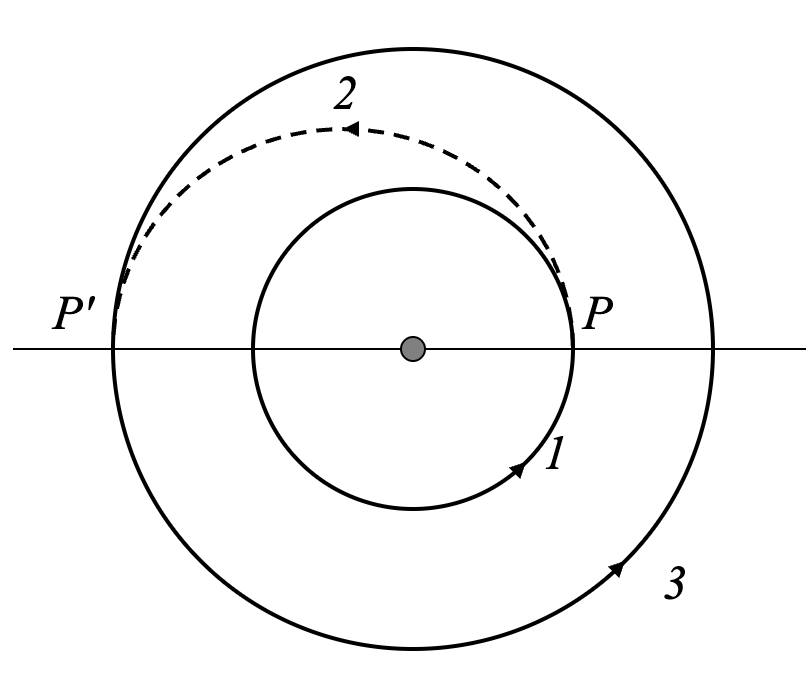
\includegraphics[width=0.3\textwidth]{transfer.png}
    \label{P7}
\end{figure}

\subsection*{Answer}

\subsubsection*{(1) Thrust factor $\lambda$ for the first boost (6 points)}
\begin{itemize}
    \item \textbf{Identify parameters for the initial circular orbit and transfer orbit:} \\
    For the initial circular orbit (Orbit 1), $c_1 = R_1$ and $\epsilon_1 = 0$. \\
    Since the velocity is boosted by $\lambda$ ($v_p = \lambda v_1$) at the same radius $R_1$, and given $c \propto L^2 \propto v^2$, the parameter $c_2$ for the transfer orbit is:
    \[
    c_2 = \lambda^2 c_1 = \lambda^2 R_1
    \]
    \hfill \textbf{(2 points)}

    \item \textbf{Relate eccentricity $\epsilon_2$ to $\lambda$ at perigee ($P$):} \\
    Point $P$ is the perigee of the transfer orbit. Using the orbit equation at $\phi=0$:
    \[
    R_1 = \frac{c_2}{1 + \epsilon_2} \implies 1 + \epsilon_2 = \frac{\lambda^2 R_1}{R_1} = \lambda^2 \implies \epsilon_2 = \lambda^2 - 1
    \]
    \hfill \textbf{(1 point)}

    \item \textbf{Apply condition at apogee ($P'$) to solve for $\lambda$:} \\
    Point $P'$ is the apogee of the transfer orbit where $r = R_3$. Using the orbit equation at $\phi=\pi$:
    \[
    R_3 = \frac{c_2}{1 - \epsilon_2} = \frac{\lambda^2 R_1}{1 - (\lambda^2 - 1)} = \frac{\lambda^2 R_1}{2 - \lambda^2}
    \]
    \hfill \textbf{(2 points)} \\
    \textit{(1 point for the apogee equation formula, 1 point for correct substitution)}

    \item \textbf{Calculate the final value:} \\
    Given $R_3 = 2R_1$, substitute and solve:
    \[
    2 = \frac{\lambda^2}{2 - \lambda^2} \implies 4 - 2\lambda^2 = \lambda^2 \implies 3\lambda^2 = 4
    \]
    \[
    \lambda = \sqrt{\frac{4}{3}} \approx 1.15
    \]
    \hfill \textbf{(1 point)}
\end{itemize}

\subsubsection*{(2) Thrust factor $\lambda'$ for the second boost (6 points)}
\begin{itemize}
    \item \textbf{Determine parameters for the final circular orbit (Orbit 3):} \\
    For the final circular orbit of radius $R_3$, the parameter $c_3$ is simply the radius itself (since $\epsilon=0$):
    \[
    c_3 = R_3
    \]
    \hfill \textbf{(1 point)}

    \item \textbf{Method A: Using Ratio of Angular Momenta / Parameters (Recommended):} \\
    The thrust factor is the ratio of velocities at the same radius $R_3$: $\lambda' = v_3 / v_{p'}$.
    Since $L = m R_3 v$, the velocity ratio is equal to the angular momentum ratio:
    \[
    \lambda' = \frac{L_3}{L_2}
    \]
    Using the definition $c \propto L^2$, we have $\frac{L_3}{L_2} = \sqrt{\frac{c_3}{c_2}}$.
    \hfill \textbf{(3 points)} \\
    \textit{(Alternatively, \textbf{Method B}: Calculate $v_3 = \sqrt{GM/R_3}$ and $v_{p'}$ using conservation of energy/angular momentum, and take the ratio. Award full points for correct logic.)}

    \item \textbf{Substitute and Solve:} \\
    Using $c_3 = R_3 = 2R_1$ and $c_2 = \lambda^2 R_1 = \frac{4}{3}R_1$ (from Part 1):
    \[
    \lambda' = \sqrt{\frac{R_3}{c_2}} = \sqrt{\frac{2R_1}{4/3 R_1}} = \sqrt{\frac{6}{4}} = \sqrt{\frac{3}{2}}
    \]
    \hfill \textbf{(2 points)} \\
\end{itemize}

\newpage
\section*{Problem 8 [$6 + 10$ points]}
\begin{enumerate}
\item[(1)]  What are the conditions on the ``small" constants $a$, $b$, $c$, $d$, $e$, and $f$ in order that 
\begin{equation*}
    q= Q+ aQ^2+2bQP + cP^2
\end{equation*}
\begin{equation*}
   p=P+dQ^2+2eQP+fP^2
\end{equation*}
be canonical transformation to \textbf{first order} in small quantities?

\item[(2)] The Hamiltonian for a slightly anharmonic oscillator is 
\begin{equation*}
   H=\frac{p^2}{2m} + \frac{1}{2}m\omega^2q^2 + \beta q^3
\end{equation*}
where $\beta$ is ``small". Perform a canonical transformation of the type given in (1) and adjust the constants so that the new Hamiltonian $H$ does not contain an anharmonic term to first order in small quantities, thus 
\begin{equation*}
   H'=\frac{P^2}{2m} + \frac{1}{2}m\omega^2Q^2 + ...
\end{equation*}
Write down the transformations rules between $(q, p)$ and $(Q, P)$.
\end{enumerate}

\subsection*{Answer}

\subsubsection*{(1) Conditions for Canonical Transformation (6 points)}
\begin{itemize}
    \item \textbf{Method Identification:} Recognize that for the transformation to be canonical, the fundamental Poisson bracket must be unity:
    \[ [q, p]_{Q,P} = \frac{\partial q}{\partial Q}\frac{\partial p}{\partial P} - \frac{\partial q}{\partial P}\frac{\partial p}{\partial Q} = 1 \]
    \hfill \textbf{(2 points)}
    
    \item \textbf{Calculation and Linearization:} Calculate the partial derivatives and multiply them, keeping only terms to the \textbf{first order} in small constants ($a, b, \dots, f$).
    \begin{align*}
        \frac{\partial q}{\partial Q} &= 1 + 2aQ + 2bP, & \frac{\partial q}{\partial P} &= 2bQ + 2cP \\
        \frac{\partial p}{\partial Q} &= 2dQ + 2eP, & \frac{\partial p}{\partial P} &= 1 + 2eQ + 2fP
    \end{align*}
    Substitution yields:
    \[ [q, p] \approx (1 + 2aQ + 2bP)(1 + 2eQ + 2fP) - (0)(0) \approx 1 + 2(a+e)Q + 2(b+f)P \]
    \textit{(Note: Cross terms like $(2bQ)(2dQ)$ are second order and vanish.)}
    \hfill \textbf{(2 points)}
    
    \item \textbf{Final Conditions:} Set the coefficients of $Q$ and $P$ to zero to satisfy $[q, p] = 1$:
    \[ a + e = 0 \quad \text{and} \quad b + f = 0 \]
    \hfill \textbf{(2 points)}
\end{itemize}

\subsubsection*{(2) Removing the Anharmonic Term (10 points)}
\begin{itemize}
    \item \textbf{Hamiltonian Expansion:} Substitute the expressions for $q(Q,P)$ and $p(Q,P)$ into the Hamiltonian $H = \frac{p^2}{2m} + \frac{1}{2}m\omega^2q^2 + \beta q^3$. Expand and group terms by powers of $Q$ and $P$, keeping only first-order small quantities.
    \[ H(Q,P) = \underbrace{\frac{P^2}{2m} + \frac{1}{2}m\omega^2Q^2}_{\text{Zero order}} + \underbrace{\dots}_{\text{First order corrections}} \]
    Key expansion terms needed:
    \begin{itemize}
        \item Coeff of $Q^3$: $m\omega^2 a + \beta$
        \item Coeff of $Q^2P$: $\frac{d}{m} + 2m\omega^2 b$
        \item Coeff of $QP^2$: $\frac{2e}{m} + m\omega^2 c$
        \item Coeff of $P^3$: $\frac{f}{m}$
    \end{itemize}
    \hfill \textbf{(3 points)} \\
    \textit{(1 point for correct substitution, 2 points for correctly grouping the coefficients)}

    \item \textbf{Setting Coefficients to Zero:} Require the new Hamiltonian to be simple harmonic ($H' = \frac{P^2}{2m} + \frac{1}{2}m\omega^2Q^2$). Thus, all anharmonic coefficients must vanish:
    \[
    \frac{f}{m} = 0, \quad m\omega^2 a + \beta = 0, \quad \frac{d}{m} + 2m\omega^2 b = 0, \quad \frac{2e}{m} + m\omega^2 c = 0
    \]
    \hfill \textbf{(2 points)}

    \item \textbf{Solving for Constants:} Combine these equations with the canonical conditions from Part (1) ($a=-e, b=-f$) to solve for all constants:
    \begin{enumerate}
        \item $f=0 \implies b=0$
        \item $b=0 \implies d=0$
        \item $m\omega^2 a + \beta = 0 \implies a = -\frac{\beta}{m\omega^2}$
        \item $a = -e \implies e = \frac{\beta}{m\omega^2}$
        \item $c = -\frac{2e}{m^2\omega^2} = -\frac{2\beta}{m^3\omega^4}$
    \end{enumerate}
    \hfill \textbf{(3 points)} \\
    \textit{(Partial credit if only some constants are correct)}

    \item \textbf{Final Transformation Rules:} Write the final explicit transformations:
    \[
    q = Q - \frac{\beta}{m\omega^2}Q^2 - \frac{2\beta}{m^3\omega^4}P^2 \quad \left( \text{or } Q - \frac{\beta}{m\omega^2}\left(Q^2 + \frac{2P^2}{m^2\omega^2}\right) \right)
    \]
    \[
    p = P + \frac{2\beta}{m\omega^2}QP
    \]
    \hfill \textbf{(2 points)}
\end{itemize}


\newpage
\section*{Problem 9 [$12$ points ]}
A pendulum consists of a mass $m$ at the end of a massless stick of length $l$. The other end of the stick is made to oscillate vertically with a position given by $y(t) = A \cos(\omega t)$, where $A \ll l$. It turns out that if $\omega$ is large enough, and if the pendulum is initially nearly upside-down, then surprisingly it will not fall over as time goes by. Find the equation of motion for the angle of the pendulum (measured relative to its upside-down position). You may simply the final equation of motion using the small-angle approximation.

\begin{figure}[h]
    \centering
    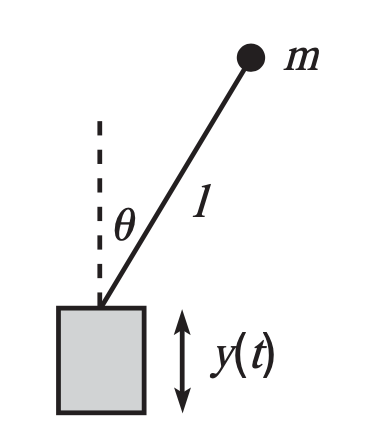
\includegraphics[width=0.3\textwidth]{invertedPendulum.png}
    \label{P7}
\end{figure}

\subsection*{Answer}

\subsubsection*{(1) Lagrangian Formulation (4 points)}
\begin{itemize}
    \item \textbf{Coordinates \& Velocity Setup:}
    Define the position of the mass $m$ relative to a fixed inertial frame. With the pivot moving at $y(t)$ and angle $\theta$ measured from the vertical upward:
    \[
    X = l \sin \theta, \quad Y = y(t) + l \cos \theta
    \]
    Calculate the velocity squared $v^2 = \dot{X}^2 + \dot{Y}^2$:
    \[
    v^2 = l^2 \dot{\theta}^2 + \dot{y}^2 - 2 l \dot{y} \dot{\theta} \sin \theta
    \]
    \hfill \textbf{(2 points)} \\
    
    \item \textbf{Lagrangian ($L$):}
    Write down the kinetic energy $T = \frac{1}{2}m v^2$ and potential energy $V = mgY = mg(y + l \cos \theta)$. Construct $L = T - V$:
    \[
    L = \frac{1}{2}m(l^2 \dot{\theta}^2 + \dot{y}^2 - 2 l \dot{y} \dot{\theta} \sin \theta) - mg(y + l \cos \theta)
    \]
    \hfill \textbf{(2 points)}
\end{itemize}

\subsubsection*{(2) Derivation of Euler-Lagrange Equation (4 points)}
\begin{itemize}
    \item \textbf{Canonical Momentum \& Time Derivative:}
    Calculate the partial derivative with respect to $\dot{\theta}$ and its time derivative:
    \[
    \frac{\partial L}{\partial \dot{\theta}} = m l^2 \dot{\theta} - m l \dot{y} \sin \theta
    \]
    \[
    \frac{d}{dt}\left( \frac{\partial L}{\partial \dot{\theta}} \right) = m l^2 \ddot{\theta} - m l (\ddot{y} \sin \theta + \dot{y} \dot{\theta} \cos \theta)
    \]
    \hfill \textbf{(2 points)} \\
    \textit{(Crucial step: correctly applying the chain rule to $\frac{d}{dt}(\dot{y} \sin \theta)$)}

    \item \textbf{Generalized Force \& Combination:}
    Calculate $\frac{\partial L}{\partial \theta}$:
    \[
    \frac{\partial L}{\partial \theta} = - m l \dot{y} \dot{\theta} \cos \theta + mgl \sin \theta
    \]
    Apply the Euler-Lagrange equation. Notice that the terms involving $\dot{y}\dot{\theta}\cos\theta$ cancel out:
    \[
    m l^2 \ddot{\theta} - m l \ddot{y} \sin \theta - mgl \sin \theta = 0 \implies l \ddot{\theta} - \ddot{y} \sin \theta = g \sin \theta
    \]
    \hfill \textbf{(2 points)}
\end{itemize}

\subsubsection*{(3) Specific Solution and Approximation (4 points)}
\begin{itemize}
    \item \textbf{Substitute Explicit $y(t)$:}
    Calculate the acceleration of the support from $y(t) = A \cos(\omega t)$:
    \[
    \ddot{y} = -A \omega^2 \cos(\omega t)
    \]
    Substitute $\ddot{y}$ into the equation of motion:
    \[
    l \ddot{\theta} - (-A \omega^2 \cos(\omega t)) \sin \theta = g \sin \theta
    \]
    Rearrange to group terms:
    \[
    l \ddot{\theta} + \sin \theta (A \omega^2 \cos(\omega t) - g) = 0
    \]
    \hfill \textbf{(2 points)}

    \item \textbf{Small Angle Approximation:}
    Apply the small angle approximation $\sin \theta \approx \theta$.
    \[
    l \ddot{\theta} + \theta (A \omega^2 \cos(\omega t) - g) = 0
    \]
    Or in the form shown in the reference (dividing by $l$):
    \[
    \ddot{\theta} + \theta \left( \frac{A}{l} \omega^2 \cos(\omega t) - \frac{g}{l} \right) = 0
    \]
    \hfill \textbf{(2 points)}
\end{itemize}

\newpage
\section*{Bonus Problem 10 [$10$ points]}
Consider a particle of mass $m$ and electric charge $q$ moving in the presence of time-dependent electromagnetic fields. The particle's motion is described by the relativistic Lagrangian:
\[
L = -mc^2\sqrt{1 - \frac{v^2}{c^2}} + q\, \mathbf{v} \cdot \mathbf{A}(\mathbf{r}, t) - q\, V(\mathbf{r}, t),
\]
where $\mathbf{v} = \dv{\mathbf{r}}{t}$ is the particle's velocity; $V(\mathbf{r}, t)$ is the scalar potential; $\mathbf{A}(\mathbf{r}, t)$ is the vector potential; $c$ is the speed of light. Take the non-relativistic limit by expanding the Lagrangian to leading order in $v/c$ (i.e., assume $v \ll c$). From the resulting approximate Lagrangian, derive the equation of motion.
Hint: $\mathbf{E} = -\nabla V - \pdv{\mathbf{A}}{t}$ and $\mathbf{B} = \nabla \times \mathbf{A}$.

\subsection*{Answer}
\subsubsection*{(1) Non-Relativistic Approximation (3 points)}
\begin{itemize}
    \item Expand the relativistic term $\sqrt{1 - v^2/c^2}$ using the Taylor series $(1-x)^{1/2} \approx 1 - x/2$:
    \[
    -mc^2\sqrt{1 - \frac{v^2}{c^2}} \approx -mc^2\left(1 - \frac{v^2}{2c^2}\right) = -mc^2 + \frac{1}{2}mv^2
    \]
    \hfill \textbf{(1 point)}
    \item Write down the approximate non-relativistic Lagrangian. Note that the constant term $-mc^2$ can be dropped as it does not affect the equations of motion (though keeping it is also correct):
    \[
    L \approx \frac{1}{2}mv^2 + q\, \mathbf{v} \cdot \mathbf{A} - q\, V
    \]
    \hfill \textbf{(2 points)} \\
\end{itemize}

\subsubsection*{(2) Euler-Lagrange Derivatives (4 points)}
\begin{itemize}
    \item \textbf{Time Derivative Term:}
    Calculate the canonical momentum $\pdv{L}{\mathbf{v}}$ and its total time derivative.
    \[ \frac{\partial L}{\partial \mathbf{v}} = m\mathbf{v} + q\mathbf{A} \]
    Compute $\frac{d}{dt}(\frac{\partial L}{\partial \mathbf{v}})$, correctly applying the chain rule to $\mathbf{A}(\mathbf{r}, t)$:
    \[ \frac{d}{dt}(m\mathbf{v} + q\mathbf{A}) = m\dot{\mathbf{v}} + q\left( \frac{\partial \mathbf{A}}{\partial t} + (\mathbf{v} \cdot \nabla)\mathbf{A} \right) \]
    \hfill \textbf{(2 points)} \\

    \item \textbf{Spatial Derivative Term:}
    Calculate the gradient $\pdv{L}{\mathbf{r}}$. Use vector identity $\nabla(\mathbf{v} \cdot \mathbf{A}) = (\mathbf{v} \cdot \nabla)\mathbf{A} + \mathbf{v} \times (\nabla \times \mathbf{A})$ (treating $\mathbf{v}$ as constant independent of $\mathbf{r}$):
    \[ \frac{\partial L}{\partial \mathbf{r}} = q\nabla(\mathbf{v} \cdot \mathbf{A}) - q\nabla V = q\left[ (\mathbf{v} \cdot \nabla)\mathbf{A} + \mathbf{v} \times (\nabla \times \mathbf{A}) \right] - q\nabla V \]
    \hfill \textbf{(2 points)} \\
\end{itemize}

\subsubsection*{(3) Final Equation of Motion (3 points)}
\begin{itemize}
    \item \textbf{Assembly and Cancellation:}
    Equate the time derivative term to the spatial derivative term:
    \[ m\dot{\mathbf{v}} + q\frac{\partial \mathbf{A}}{\partial t} + q(\mathbf{v} \cdot \nabla)\mathbf{A} = q(\mathbf{v} \cdot \nabla)\mathbf{A} + q\mathbf{v} \times (\nabla \times \mathbf{A}) - q\nabla V \]
    Show that the term $q(\mathbf{v} \cdot \nabla)\mathbf{A}$ cancels out on both sides.
    \hfill \textbf{(1 point)}
    
    \item \textbf{Field Identification:}
    Rearrange the terms and substitute the definitions $\mathbf{B} = \nabla \times \mathbf{A}$ and $\mathbf{E} = -\nabla V - \pdv{\mathbf{A}}{t}$:
    \[ m\dot{\mathbf{v}} = q\left( -\nabla V - \frac{\partial \mathbf{A}}{\partial t} \right) + q\mathbf{v} \times (\nabla \times \mathbf{A}) \]
    \hfill \textbf{(1 point)}
    
    \item \textbf{Result:}
    Arrive at the Lorentz force law:
    \[ m\dot{\mathbf{v}} = q(\mathbf{E} + \mathbf{v} \times \mathbf{B}) \quad \text{or} \quad \mathbf{F} = q(\mathbf{E} + \mathbf{v} \times \mathbf{B}) \]
    \hfill \textbf{(1 point)}
\end{itemize}


\end{document}